\documentclass[conference]{IEEEtran}
\IEEEoverridecommandlockouts
% The preceding line is only needed to identify funding in the first footnote. If that is unneeded, please comment it out.
\usepackage{cite}
\usepackage{amsmath,amssymb,amsfonts}
\usepackage{algorithmic}
\usepackage{graphicx}
\usepackage{textcomp}
\usepackage{xcolor}
\usepackage{nameref}
\usepackage{autoref}
\usepackage{hyperref}
\usepackage{listings}
\def\BibTeX{{\rm B\kern-.05em{\sc i\kern-.025em b}\kern-.08em
    T\kern-.1667em\lower.7ex\hbox{E}\kern-.125emX}}
\newcommand*{\fullref}[1]{\textit{\hyperref[{#1}]{\autoref*{#1} \nameref*{#1}}}}

\begin{document}
\title{Duplicate recognition for restaurant dataset*\\
	{\footnotesize \textsuperscript{*}}
}
\author{\IEEEauthorblockN{1\textsuperscript{st} Alexander Christoph}
	\IEEEauthorblockA{\textit{OTH Regensburg} \\
		Regensburg, Germany \\
		alexander.christoph@st.oth-regensburg.de}
}


\maketitle

\begin{abstract}
This document describes the analysis and removal of duplicates from the restaurants dataset\cite{bib:dataset}. The aim is to remove as many duplicates as possible from this data and store it in a cloud hosted mongodb instance without duplicates. A problem when searching for duplicated entries of restaurants (or nearly any other dataset) is the format and the different writing of the entries in the data. This problem was already researched by several IEEE members\cite{bib:foreign_research}. Within my research I used different approaches to preprocess and detect duplicates. The accuracy of my results is measured with the metrics accuracy, precision and recall. After removing duplicates, the cleared dataset is stored into a mongodb cluster so that it can be accessed any time.
\end{abstract}

\begin{IEEEkeywords}
duplicate detection, restaurant dataset
\end{IEEEkeywords}

\section{Introduction}
In times where big data gets more and more attraction from the industry, it is very important to learn how to deal with it. Especially when it comes to the structure and format of the data. When looking at big data, it is most of the time a problem that there are duplicates and unclean entries in a dataset. This gives inaccurate results when analyzing or working with that data. This happens because most of the time there isn't that much preprocessing happening and there aren't even checks for a standard data format. To learn how to deal with duplicated entries, the restaurants dataset is used. This isn't actually big data, but to understand the importance of the preprocessing task, it is pretty good because it's considered a well researched data set to play with and compare to the gold standard. 

In this research, the focus was on how to preprocess the data to detect as many duplicated entries as possible and remove them from the data set. The hard task was to find ways to prepare the data so that duplicates can be found easily. In order to achieve this, generic cleansing processes, which apply to each column of the data were first used. Then each column was considered individually and specific methods were applied to them.

Once the entire clearing process was completed, ways of finding duplicates had to be investigated. For this purpose, it was chosen that an entry will be recognized as duplicate if a certain column combination had exactly the same values as another entry.

In order to measure the results achieved, various metrics such as accuracy, recall and precision were used (see \fullref{sec:metrics}). The achieved metrics can be found in \fullref{tab:results}

A cloud-hosted mongodb cluster was used to store the resulting data set.
\section{Why duplicate detection is important}
Duplicate recognition is an important task in data science for several reasons. When a data scientist receives data for research, it is often a problem that the data is not pre-processed and contains incorrect or duplicated entries. Detecting and removing these is a difficult but important task. If you work with impure data, errors can happen. For example, let's look at the restaurant record described in \fullref{sec:dataset}. This data can be used to recommend restaurants to an user of an application. If the recommendation contains duplicates with even different spelling for the same restaurant, the user could get confused and stop using our application. Duplicate detection is also important when solving machine learning tasks because most machine learning algorithms cannot handle duplicates and therefore give higher priority to duplicate records, which would result in a less accurate machine learning model.

Because of these problems, duplicate recognition is such a big issue in the field of computer science.
\section{The restaurants data set} \label{sec:dataset}
The restaurants data set investigated in this thesis is a .tsv data set describing the location and type of different restaurants. It contains 864 rows of data with six columns. The columns of the record are: 
\begin{itemize}
	\item id: The unique id of each row
	\item name: The name of the restaurant
	\item address: The address where the restaurant is located
	\item city: The city of the restaurant
	\item phone: The phone number of the restaurant
	\item type: The kind of the restaurant (i.e. french or american)
\end{itemize}
There are 122 duplicated restaurants in the data. These duplicates were hand-selected by some researchers to define a gold standard that provides the best possible result after removing all duplicates\cite{bib:reach_for_gold}. These duplicates have different variations from each other. For example, some have a different order of words in their name field, such as "the palm" and "palm the". Others have different separators for the phone number like "310/659-9639" and "310-659-9639". Sometimes the duplicate city field is a district of a larger city and sometimes it is the city name itself, like "los angeles" and "hollywood". There are more different variations in the data set, the solution of which is discussed later in the section \fullref{sec_methods} for recognition.

This investigation focused mainly on the name, city, address and phone columns, as these have the most useful information for duplicate recognition, while the id column was omitted because it is only a unique identifier that would not be useful for duplicate recognition. The type column was omitted because there were too many restaurants of the same type, which would result in an unclean target record.

In addition to the pure restaurant record, a second record, which contains all duplicates of the data per id is also specified. In this duplicate record there are only two columns, "id1" and "id2", which define the original and the duplicate id. A record without all these duplicates is considered a gold standard. The achieved results were measured according to this gold standard.
\section{Metrics used to measure results} \label{sec:metrics}
To measure the accuracy of the results of duplicate recognition, there are various metrics that are commonly used. For all these, it is important to pre-calculate four values using the gold standard data and the archived results:  
\begin{itemize}
	\item True positives (TP): The correct classified true entries
	\item True negatives (TN): The correct classified false entries
	\item False positives (FP): Incorrect classified true entries
	\item False negatives (FN): Incorrect classified false entries
\end{itemize}
In a gold standard dataset there are no false positives and false negatives\cite{bib:reach_for_gold}.

A first metric that is important is the well known accuracy. 
\begin{align}
 accuracy =  \frac{TP + TN}{TP + TN + FP + FN}
\end{align}
Only the calculating the accuracy was not sufficient for this task, since it only provides reliable results if a data set is balanced. In this case, this means that there are as many duplicate entries as there are non-duplicate entries. As an addition to accuracy, two more metrics are used, precision and recall.

Precision measures the accuracy for the minority class by considering only the positive classifications of the result set. It is therefore a good measure of unbalanced data.
\begin{align}
	Precision = \frac{TP}{TP + FP}
\end{align}
Recal instead gives the accuracy for the fraction of relevant data.
\begin{align}
	Recall = \frac{TP}{TP + FN}
\end{align}
The results obtained are measured after each important step of the pre-processing task and are presented in the \fullref{sec:results}.
\section{Preprocessing the data set} \label{sec_methods}
The research was written in Python, a programming language widely used for data science tasks. The Python-Pandas framework, which provides good data analysis capabilities was used for this research\cite{bib:pandas_doc}. While the code was written, care was taken to ensure that it would work for other records in the same format. 

The goal of the methods used was to minimize the number of unique values in each column representing the same "real" value so that an equality match for different column combinations (see \fullref{sec:dup_detection_method}) could match them as duplicates.

After each step of the pre-processing pipeline, all double spaces in the strings were removed as precaution.

A complete conclusion of the pre-processing flow can be found in Fig.~\ref{fig:program_flow}
\begin{figure}[htbp]
	\centerline{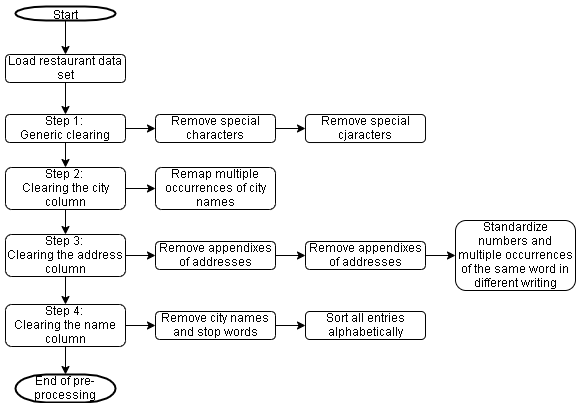
\includegraphics[width=6cm]{figures/program_flow.png}}
	\caption{Program flow}
	\label{fig:program_flow}
\end{figure}
\subsection{Studying the dataset}
The first step in data science tasks is to examine the structure and the different columns of a data set. 

This was done by looking at the first lines of the record itself and looking at the values of the different entries to understand their meaning. Afterwards it was necessary to look at each column on its own. This was done by looking at the unique values of each column in particular. Here it was found that e.g. the column type is very inconsistent with its values (i.e. sometimes the value is "Pizza" and sometimes "Italian" for the same type of restaurant) and would not fit as a column to find duplicates, because after normalization there would be too many restaurants of the same type. Therefore the column "Type" was dropped for this investigation.

The results of researching the other columns name, phone and address are described in the subsections below.
\subsection{Step 1: Generic clearing of the columns}
As a first approach it was necessary to perform as many generic operations for all columns as possible. 

Many errors in the data came from special characters. So all special characters except spaces were removed from the four columns considered (name, city, address, phone). Upper and lower case letters did not have to be considered, since all the data was in lower case. Otherwise it would have been necessary to convert all strings to lower case.

Further investigation of the alphabetic columns has shown that some values contain cardinal points and others do not. Sometimes the cardinal points were even written differently (e.g. "n" and "north"). So the next step was to write a regex that recognizes every occurrence of a cardinal point. The regex that recognizes them is: 
\begin{lstlisting}
'(( |^)((south)|(east)|(west)|(north)|
(ne)|(se)|(nw)|(sw)|s|w|e|n)( |$))'
\end{lstlisting}
This was then used to replace everything that matches with an empty string.

After applying generic data clearing, the duplicates for each column have grown. Especially for the phone column, it was noticeable that the detected duplicates have grown from seven to 116, which is quite good.
\subsection{Step 2: Clearing the city column}
After the generic clearing, it was necessary to clean up the specifics of each column on its own. It was found that some city names were written inconsistently. For example, sometimes "la" was written instead of "los angeles". So every duplicate occurrence of a city name was mapped to a default value. This map looked like: 
\begin{lstlisting}
	"la", "west la" -> "los angeles"
	"new york city" -> "new york"
\end{lstlisting}
After applying this mapping, the "city" column was considered as cleared.

When looking at the resulting metrics, it is noticeable that due to this allocation only two more duplicates were found in this column compared to the previous step. But this is okay, because the city column already contained 817 duplicates before and it is common that there aren't that many different values when viewing at restaurants that are only located at several citys.
\subsection{Step 3: Clearing the address column}
The next step was to clean up the address column. When looking at the entries, it was found that many addresses have unnecessary attachments to describe the location of a restaurant more precisely (e.g. "3125 piedmont rd. near peachtree rd."). These had to be removed from the entries. To do this, it was decided to collect the words that separate the actual address from its description and remove everything behind it. The words found were: 
\begin{lstlisting}
"between", "off", "near", "at" and "in"
\end{lstlisting}
Another inconsistency to be resolved was the different spelling of numbers (i.e. "1", "1st" or "first"). To solve this, a regex was used to detect and then remove appendages of numbers. The regex used to recognize attachments of numbers is: 
\begin{lstlisting}
'(?<=\d)(st|nd|rd|th)\b'
\end{lstlisting}
To normalize all numbers, it was subsequently necessary to map occurrences of string numbers to their numerical representation. This mapping looked like: 
\begin{lstlisting}
	first -> 1
	second -> 2
	...
	twelfth -> 12
\end{lstlisting} 
For the further cleaning of the address column it was necessary to map different occurrences of the same word to a single one. The map to accomplish this was 
\begin{lstlisting}
	"la" -> "los angeles" 
	"ave" -> "avenue"
	"rd" -> "road"
	"blv", "blvd" -> "boulevard" 
	"st" -> "street"
\end{lstlisting} 
After applying these clearing steps to the address column, the unique values have decreased from 761 to 739, and the duplicates in this particular column have increased from 116 to 125 compared to the previous step, meaning that nine more duplicated entries have been found in this column compared to the state before applying these clearing steps.
\subsection{Step 4: Clearing the name column}
The last column to be cleaned up was name. Initially, a similar procedure as for the address column was used to remove more precise descriptions for the location. So everything after the words "between", "off", "near", "at", "in" and "of" was removed.


Then it was discovered that the name of a restaurant sometimes contains the name of the city in which it is located. This information is already present in the city column and only adds noise to the data, so it was decided to remove these city names. In addition, some other words were found that would not have been useful in duplicate detection, which were also removed. So all cities in the city column and additionally "the", "restaurant", "and" and "new york city", were selected and removed. To get these so called "stop words" as regex, the following code was used: 
\begin{lstlisting}
unique_city_list = restaurant_data.city.unique()
city_regex = re.compile('the|restaurant|
and|new york city|' +'|'.join(map
(re.escape, unique_city_list)))
\end{lstlisting}
The last step was to arrange the values of the name entries alphabetically, because sometimes the restaurant names were written in different order. 

After applying these transformations to the name column, the unique values have been reduced from 773 to 746. The duplicate values in this column have increased from 91 to 118. The results that were achieved as a whole are discussed in \fullref{sec:results}.
\subsection{Duplicate detection method} \label{sec:dup_detection_method}
To detect duplicates, research has shown that most of them could be detected by selecting a combination of the columns ['address', 'name', 'phone'], ['address', 'city', 'name'] or ['name', 'city', 'phone'], in which each value must be the same to be considered a duplicate. All these three duplicate lists are then merged to obtain a complete set of duplicates from the record.
\section{Results and possible improvements}\label{sec:results}
The results obtained are displayed in \fullref{tab:results}. In total, without viewing the gold standard data set, 101 out of 112 duplicates were found in the restaurants data. This resulted in a recal of 0.90 and a precision of 1.0. 

The precision of 1.0 means that there were no false positives in our data set, which is very good. 

The recal of 0.90 means that after applying all pre-processing tasks and selecting duplicates with a combination of different columns, 90\% of the real duplicates were found.

The approach used was rather simple and could be improved e.g. by better deciding which combination of columns to use to determine if an item is a duplicate. 

Another way to improve the results could have been to better clear the "city" column, so that districts like "hollywood" are mapped to the city they belong to. 

Several researchers from the IEEE researched the issue of duplicate record detection and showed lots of different techniques to detect duplicates. They also tried a machine learning approach\cite{bib:foreign_research}.   
\begin{table}[h]
	\begin{center}
		\caption{Metrics for the reached results}
		\label{tab:results} 
		\begin{tabular}{|p{1.5cm}||p{0.8cm}|p{0.8cm}|p{0.8cm}|p{0.8cm}|p{0.8cm}|}
			\hline
			Metric & At beginning & After step 1 & After step 2 & After step 3 & After step 4 \\ 
			\hline\hline
			Dupliactes in address &92&116&116&125&125\\
			\hline
			Dupliactes in name &88&91&91&91&118\\
			\hline
			Dupliactes in city &815&817&819&819&819\\
			\hline
			Dupliactes in phone &7 & 116&116&116&116\\
			\hline
			Detected duplicates &24&68&82&83&101\\
			\hline
			True Positives &24&68&82&83&101  \\ 
			\hline
			True Negatives &752&752&752&752&11  \\  
			\hline
			False Positives &0&0&0&0&0\\  
			\hline
			False Negatives &88 &44&30&29&21\\  
			\hline
			Accuracy &0.9&0.95&0.97&0.97&0.99\\  
			\hline
			Precision &1.0 & 1.0&1.0&1.0&1.0\\  
			\hline
			Recall &0.21&0.61&0.73&0.74&0.90\\
			\hline
		\end{tabular}
	\end{center}
\end{table}
\section{Storing data into mongodb}
After researching and achieving a reliable result, it was important to store the obtained  data somewhere. For this purpose, a cloud-hosted mongodb database was chosen. This was done because it is easy to use and mongodb is easily populated from python. With mongodb it is possible to simply push python dictionaries into the database to store them correctly and reliably. The cloud hosting approach was chosen to be able to access the data anytime and anywhere. 


Before the collected data was sent to mongodb cluser, it was necessary to change the resulting entries back to more readable values, because in the pre-processing tasks many changes were made to the data, which made them almost unreadable for humans. It was decided to select the first entry for a duplicate from the original data and append the values of "address", "city" and "phone" from the duplicate if they differ from the original. To decide whether one of the columns is the same, the pre-processed data was used.

\section{Conclusion}
In this thesis I have presented my results of duplicate recognition with the restaurant data set. This research was done on a learning basis, so the methods used are rather naive and can be improved. While writing this report, I have gained a clear understanding of why the task of duplicate recognition is so important and so difficult to achieve.

Either way, the results obtained with an precision of 1.0 and a Recal of 0.9 for this data set are really good. Especially because there are no false positive results, which would have been a big disadvantage in this research.

This report has not focused on performance. Many of the methods used could be improved so that the script works better with large amounts of data. One way to improve performance could be to use the mongodb aggregation framework, which is very powerful and could be used for many tasks in the preprocessing pipeline instead of the Pandas library. Another improvement would be the implementation of multi-threading, since many preprocessing tasks could easily be executed on multiple compute units.

For further researches in this topic it would be intersesting to look into machine learning methods that could solve this issue. The other research which was refered in this paper\cite{bib:foreign_research} already looked into different methods to solve duplicate detection with machine learning. This report is from 2007, so a similar approach while using new machine learning algorithms could be a possible next step.

A complete code example of the steps done can be found at: https://github.com/alch94/dmdb\_duplicate\_recognition

\begin{thebibliography}{00}
	\bibitem{bib:pandas_doc} "Python pandas library documentation", Accessed on: Jan. 9, 2020.[online]. Available: https://pandas.pydata.org/pandas-docs/stable/
	\bibitem{bib:dataset} "Restaurants dataset", Accessed on: Jan 9, 2020.[online]. Available: https://hpi.de/naumann/projects/repeatability/datasets/restaurants-dataset.html
	\bibitem{bib:foreign_research} Ahmed K., Panagiotis G. and Vassilios S., "Duplicate Record Detection: A Survey", IEEE Transactions on knowledge and data engineering, vol. 19, no. 1, January 2007. Accessed on: Jan. 9, 2020.[Online]. Available: https://www.cs.purdue.edu/homes/ake/pub/TKDE-0240-0605-1.pdf
	\bibitem{bib:reach_for_gold} Tobias V., Arvid H., Uwe D., Dustin L. and Felix N., "Reach for gold: An annealing standard to evaluate duplicate detection results" Journal of Data and Information Quality (JDIQ), No. 5, September 2014. Accessed on: Jan. 9, 2020.[Online]. Available: https://dl.acm.org/doi/10.1145/2629687
\end{thebibliography}
\end{document}